\documentclass[%
%10pt,
%varwidth=false,
%crop=true,
border={0mm 0mm 0mm 0mm}]{standalone}
\usepackage[T1]{fontenc}
\usepackage[utf8]{inputenc}
\usepackage[auto]{microtype}
%\usepackage{cmbright}
\usepackage{arev}
\usepackage{amsmath, amssymb, amsfonts, icomma}
\usepackage[version=4]{mhchem}
\usepackage{tikz}
\usetikzlibrary{positioning, matrix}
\usepackage{chemplants-tub}
\usepackage{xcolor}
%define stream tip, default is stealth
\setchpstreamtip{latex}
\setchpmainstreamthickness{thick}
%\setchpunitthickness{very thick}

\pgfdeclarelayer{bg}    % declare background layer
\pgfsetlayers{bg,main}  % set the order of the layers (main is the standard layer)

\definecolor{signalgruen}{RGB}{49,127,67}    % RAL 6032 Wasser
\definecolor{signalrot}{RGB}{155,36,35}      % RAL 3001 Dampf
\definecolor{signalgrau}{RGB}{150,153,146}   % RAL 7004 Luft
\definecolor{signalgelb}{RGB}{229,190,001}   % RAL 1003 brennbare und nicht brennbare Gase
\definecolor{signalorange}{RGB}{208,93,40}   % RAL 2010 Säuren
\definecolor{signalviolett}{RGB}{132,76,130} % RAL 4008 Laugen
\definecolor{signalbraun}{RGB}{121,77,62}    % RAL 8002 brennbare und nicht brennbare Flüssigkeiten
\definecolor{signalblau}{RGB}{30,45,110}     % RAL 5005 Sauerstoff

% TABLEAU-10
\definecolor{Tab10-A}{RGB}{78, 121, 167}
\definecolor{Tab10-B}{RGB}{242, 142, 43}
\definecolor{Tab10-C}{RGB}{225, 87, 89}
\definecolor{Tab10-D}{RGB}{118, 183, 178}
\definecolor{Tab10-E}{RGB}{89, 161, 79}
\definecolor{Tab10-F}{RGB}{237, 201, 72}
\definecolor{Tab10-G}{RGB}{176, 122, 161}
\definecolor{Tab10-H}{RGB}{255, 157, 167}
\definecolor{Tab10-I}{RGB}{156, 117, 95}
\definecolor{Tab10-J}{RGB}{186, 176, 172}




\begin{document}
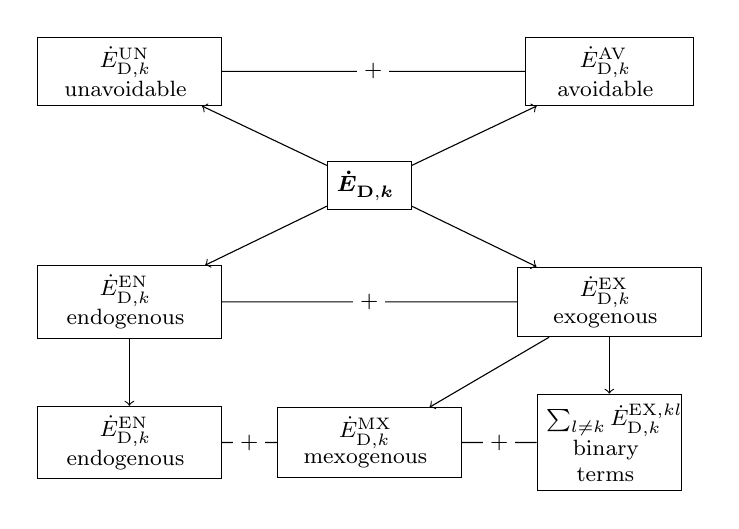
\begin{tikzpicture}[font=\footnotesize, node distance=15mm and 15mm]
  \pgfdeclarelayer{background}
  \pgfsetlayers{main,background}
  \matrix (m) [
    matrix of nodes,
    nodes={draw, align=center},
    column sep=7mm,
    row sep=7mm,
  ] {
    {\parbox{2cm}{\centering  $\dot{E}_{\text{D},k}^{\text{UN}}$ unavoidable}} & & {\parbox{1.8cm}{\centering  $\dot{E}_{\text{D},k}^{\text{AV}}$ avoidable}} \\
    & $\boldsymbol{\dot{E}}_{\mathbf{D},\boldsymbol{k}}^{}$ & \\
    {\parbox{2cm}{\centering  $\dot{E}_{\text{D},k}^{\text{EN}}$ endogenous}} & & {\parbox{2cm}{\centering  $\dot{E}_{\text{D},k}^{\text{EX}}$ exogenous}} \\
    {\parbox{2cm}{\centering  $\dot{E}_{\text{D},k}^{\text{EN}}$ endogenous}} & {\parbox{2cm}{\centering  $\dot{E}_{\text{D},k}^{\text{MX}}$ mexogenous}} & {\parbox{1.5cm}{\centering  $\sum_{l\neq k} \dot{E}_{\text{D},k}^{\text{EX},kl}$ binary terms}} \\
  };

  \begin{scope}[
    font=\footnotesize,
    inner sep=.25em,
  ]
    \draw[-]
      (m-1-1) -- node[midway, fill=white] {+} (m-1-3)
      (m-4-1) -- node[midway, fill=white] {+} (m-4-2)
      (m-4-2) -- node[midway, fill=white] {+} (m-4-3)
      (m-3-1) -- node[midway, fill=white] {+} (m-3-3);
    \draw[->]
      (m-3-3) -- (m-4-3);
    \draw[->]
      (m-3-1) -- (m-4-1);
    \draw[->]
      (m-3-3) -- (m-4-2);
    \draw[->]
      (m-2-2) -- (m-3-1);
    \draw[->]
      (m-2-2) -- (m-3-3);
    \draw[->]
      (m-2-2) -- (m-1-1);
    \draw[->]
      (m-2-2) -- (m-1-3);
  \end{scope}
\end{tikzpicture}
\end{document}

